\documentclass{article}

%% https://uwaterloo.ca/science/undergraduate/experiential-learning/
%% co-op/science-work-term-reports/work-term-report-guidelines

%%%%%%%%%%%%%%%%%%%%%%%%%%%%%%%%%%%%%%%%%%%%%%%%%%%%%%%%%%%%%%%%%%%%
%%--------------------------PREAMBLE------------------------------%%
%%%%%%%%%%%%%%%%%%%%%%%%%%%%%%%%%%%%%%%%%%%%%%%%%%%%%%%%%%%%%%%%%%%%

\usepackage[utf8]{inputenc}
\usepackage[margin=0cm]{geometry}
\usepackage{graphicx}
\graphicspath{{images/}}
\usepackage{pdfpages}
\usepackage{anyfontsize}
\usepackage{setspace}
\setcounter{section}{-1}

%%%%%%%%%%%%%%%%%%%%%%%%%%%%%%%%%%%%%%%%%%%%%%%%%%%%%%%%%%%%%%%%%%%%
%%-----------------------CUSTOM COMMANDS--------------------------%%
%%%%%%%%%%%%%%%%%%%%%%%%%%%%%%%%%%%%%%%%%%%%%%%%%%%%%%%%%%%%%%%%%%%%

\newcommand{\textBF}[1]{%
    \pdfliteral direct {2 Tr 1 w} %the second factor is the boldness
     #1%
    \pdfliteral direct {0 Tr 0 w}%
}

\newcommand{\textDF}[1]{%
    \pdfliteral direct {2 Tr 0.2 w} %the second factor is the boldness
     #1%
    \pdfliteral direct {0 Tr 0 w}%
}

%%%%%%%%%%%%%%%%%%%%%%%%%%%%%%%%%%%%%%%%%%%%%%%%%%%%%%%%%%%%%%%%%%%%
%%-----------------------DOCUMENT BEGIN---------------------------%%
%%%%%%%%%%%%%%%%%%%%%%%%%%%%%%%%%%%%%%%%%%%%%%%%%%%%%%%%%%%%%%%%%%%%

\begin{document}

\begin{titlepage}
    \thispagestyle{empty}
    \title{
        \vspace{2cm}
        
\includegraphics[width=7cm]{images/uw_logo.png} \\
        \vspace{4cm}
        \begingroup
            \setstretch{4}\fontsize{26}{10}\selectfont\fontdimen2\font=0.7ex
            \parbox{13.5cm}{\textBF{Machine Learning Principles 
            Applied to Quantum Error Correction}} % Title
        \endgroup
    }
    \date{}     % Set to empty
    \author{}   % Set to empty
    \maketitle
    \vspace{-3.5cm}
    \hspace{4cm}\parbox[b][15cm][b]{16cm}{
        \textDF{
            \large\setstretch{1.5}
            PHYS 490 -- Topics in ML\\
            \date{\today}\\
            Yusufzai, Fahim (20677986) \\
            Elkhalifa, Mujtaba (...) \\
            Bayat, Nouralhoda (...) \\
        }
    }
\end{titlepage}
\pagebreak

\newgeometry{top=1.5in,bottom=1in,right=1in,left=1.5in} 

\pagenumbering{roman}
\tableofcontents
\newpage
\listoffigures
\listoftables
\pagebreak

\section{Midterm Presentation}

The following should be included in the midterm presentation:

\begin{enumerate}

\item Fill in...

\end{enumerate}

\pagenumbering{arabic}
\section{Summary}

\begin{enumerate}
    \item purpose of the report
    \item scope of the report
    \item major points, including a summary of your research methodology
    \item highlights of the conclusions and recommendations
\end{enumerate}
\section{Introduction}

\begin{enumerate}
    \item Describe the problem or project
    \item Provide background information
    \item Clearly state the objective(s) of the report
\end{enumerate}
\section{Materials and Methods}

\begin{enumerate}
    \item Clearly describe the procedures used in your analysis, your description should allow anybody to repeat your work
    \item You can use citations to already established procedures, for example: DNA was extracted from the stool samples following the procedures described by Dumpman et al. (2016).
\end{enumerate}


\section{Results and Analysis}

\begin{enumerate}
\item Give a clear and concise presentation of the results of your analysis, incorporating figures and tables where appropriate.
\item Do not incorporate “raw” numerical data, present your data effectively using summary statistics, tables and/or figures, including charts, histograms and graphs
\end{enumerate}
\section{Discussion}

\begin{enumerate}
    \item Must include a critical analysis and overview of the material presented  in the results section
\end{enumerate}
\section{Conclusion}

\begin{enumerate}
    \item Conclusions must be supported by the analysis done in the body of the report
    \item Recommendations describe future activities that would benefit from the analysis
\end{enumerate}

``I always thought something was fundamentally wrong with the universe'' \cite{adams1995hitchhiker}

\begin{figure}[h!]
\centering
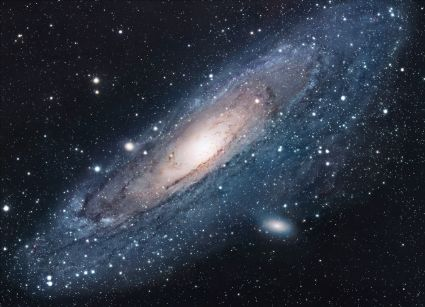
\includegraphics[scale=1.7]{../images/universe.jpg}
\caption{The Universe}
\label{fig:universe}
\end{figure}

The table \ref{table:1} is an example of referenced \LaTeX elements.
 
\begin{table}[h!]
\centering
\begin{tabular}{||c c c c||} 
 \hline
 Col1 & Col2 & Col2 & Col3 \\ [0.5ex] 
 \hline\hline
 1 & 6 & 87837 & 787 \\ 
 2 & 7 & 78 & 5415 \\
 3 & 545 & 778 & 7507 \\
 4 & 545 & 18744 & 7560 \\
 5 & 88 & 788 & 6344 \\ [1ex] 
 \hline
\end{tabular}
\caption{Table to test captions and labels}
\label{table:1}
\end{table}

\bibliographystyle{plain}
\bibliography{references}
\end{document}
